\documentclass{article}
\usepackage{fullpage}
\usepackage{graphicx}
\usepackage{tabularx}

\setlength{\parindent}{0pt}

\begin{document}

{\centering \Large \bf EECS192 Mechatronic Design Laboratory \\}
{\centering \bf Discussion 2, Car Critique Notes \\}
{\centering Compiled by: Ducky \\}

These are notes from the group car critiques conducted during the second week's discussion - thanks to all those who participated! The intention here is NOT for you to not show up to discussion (you should, otherwise this page would be empty!), but to give everyone some ideas as you work on project proposals and allow people to see what happened during the other section.

\section{Wednesday, 28 January}
\subsection{The Sonder Car}
{\centering
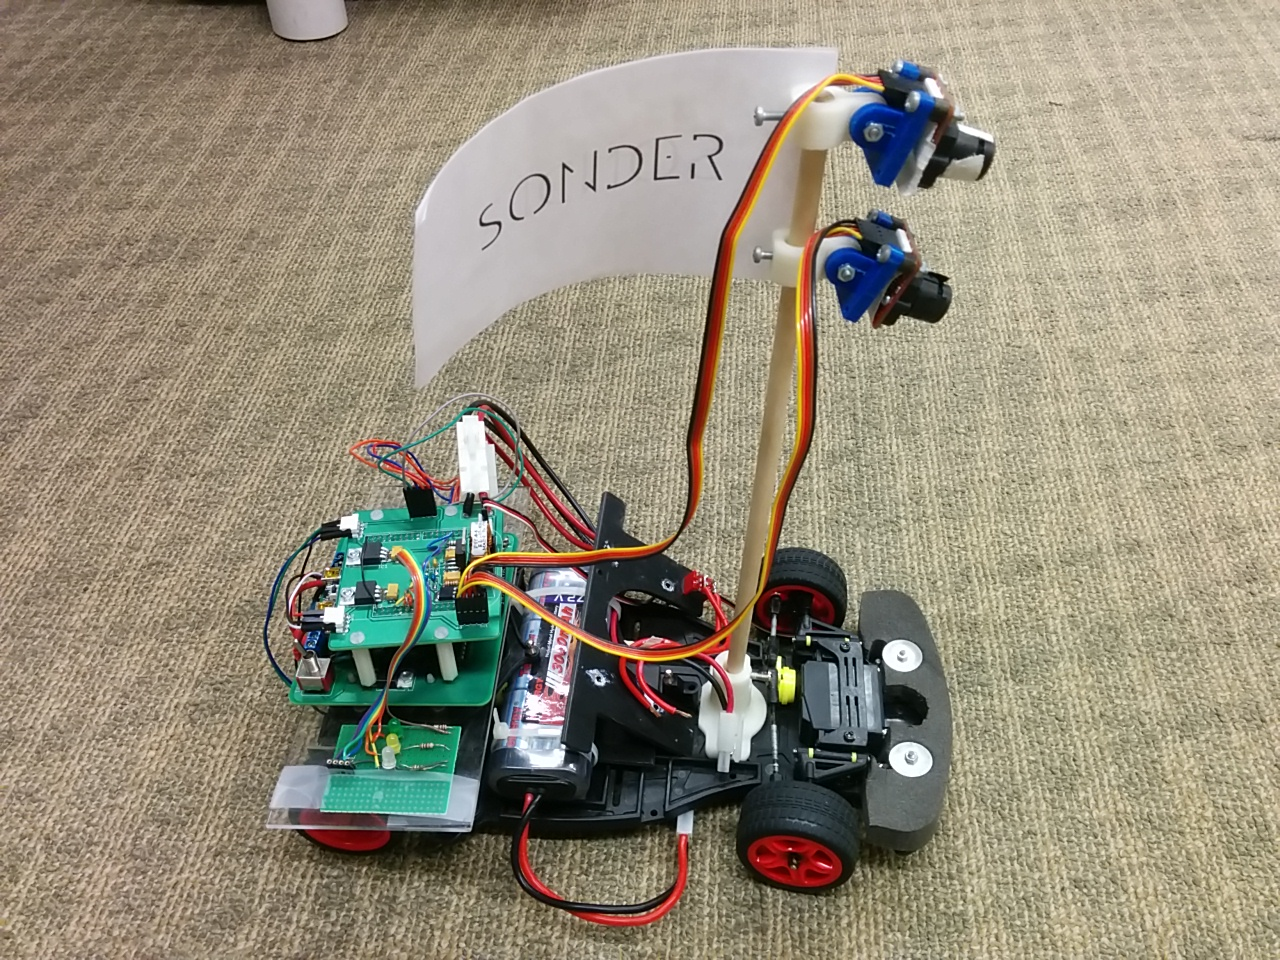
\includegraphics[width=0.32\textwidth]{images-dis2-carcritiques/sonder-side1}
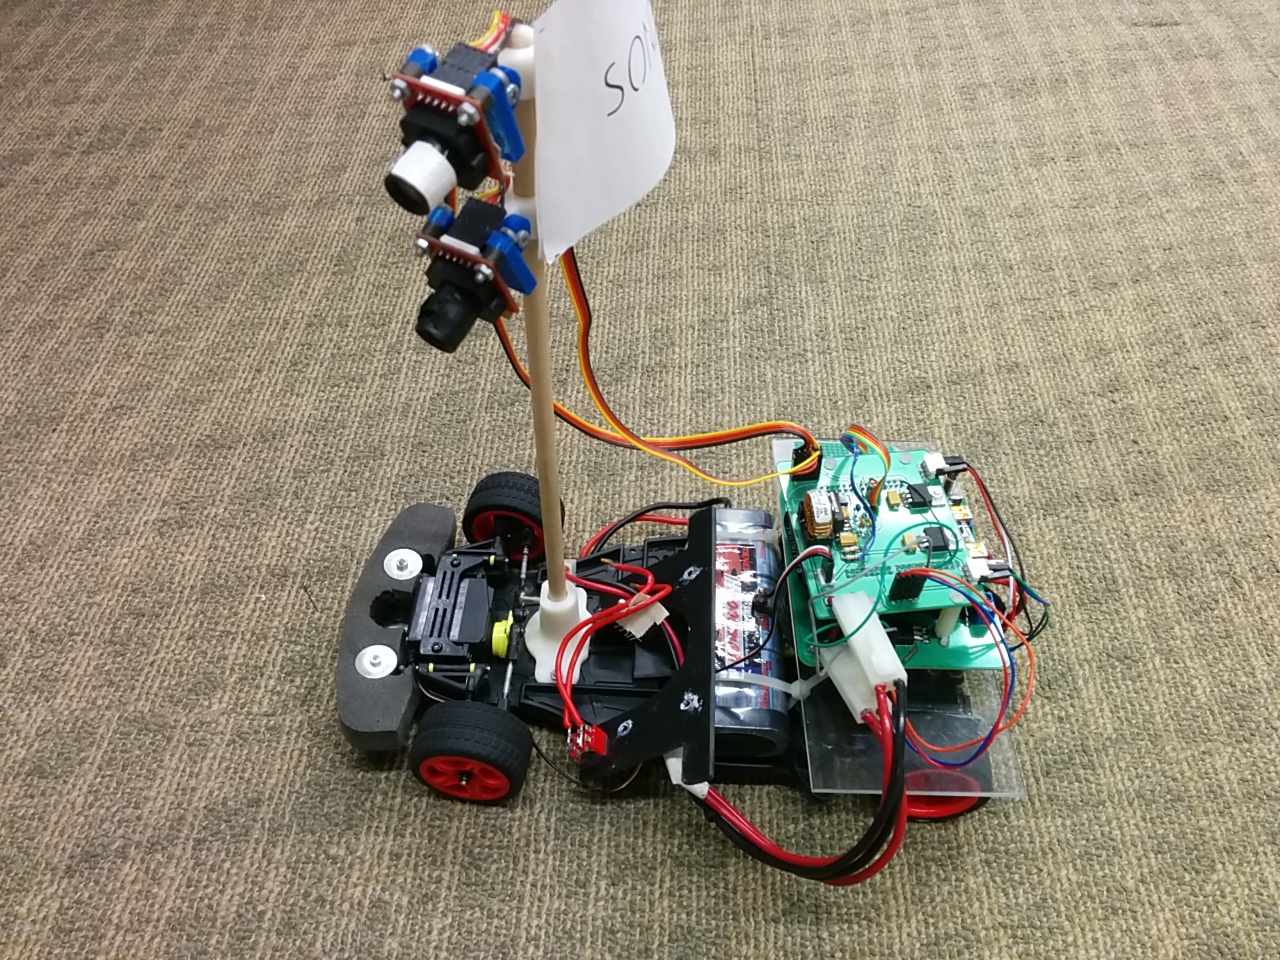
\includegraphics[width=0.32\textwidth]{images-dis2-carcritiques/sonder-side2}
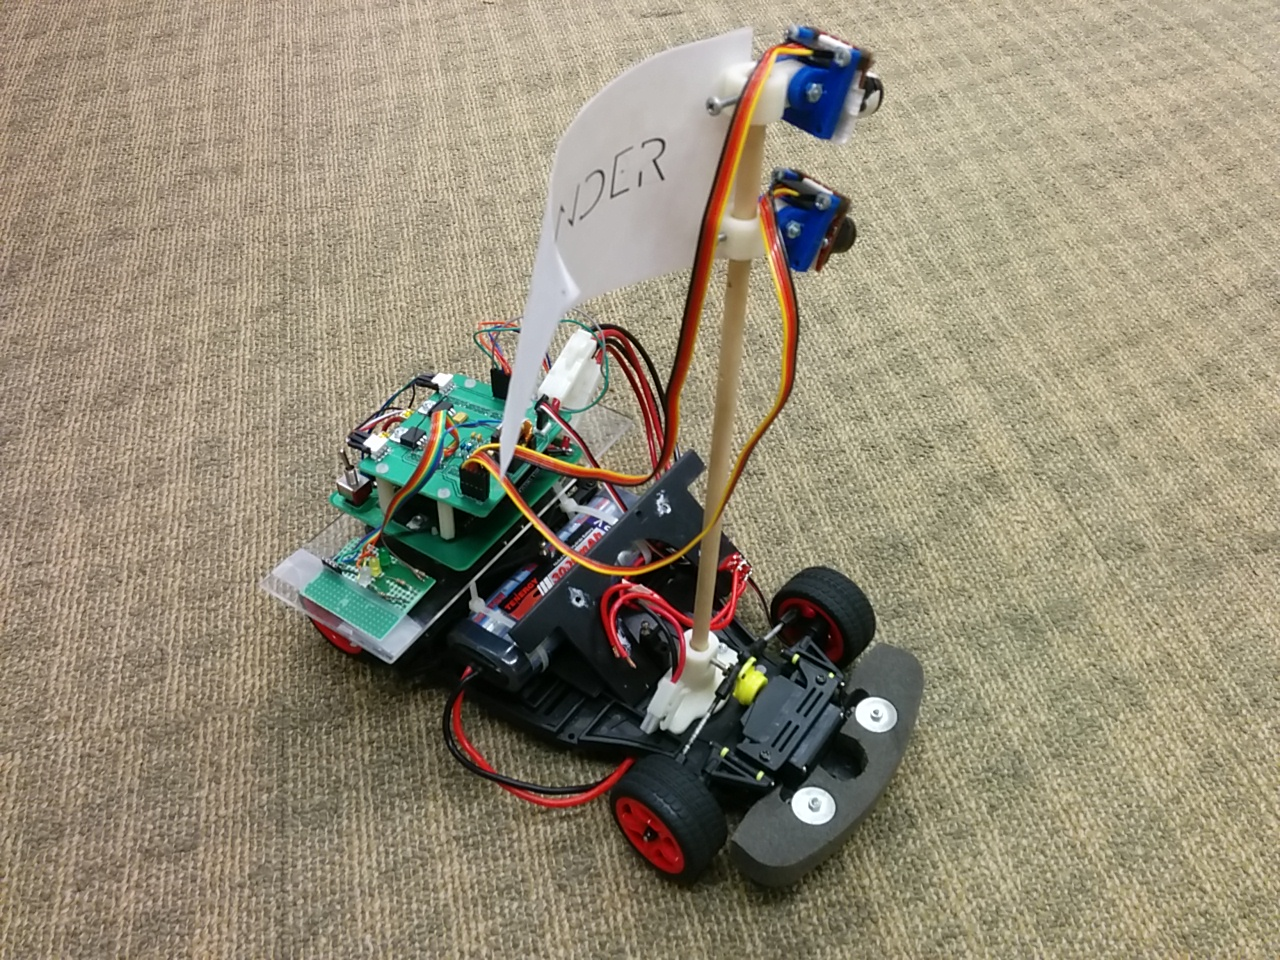
\includegraphics[width=0.32\textwidth]{images-dis2-carcritiques/sonder-angle} \\}

\begin{tabularx}{\textwidth}{X X}
\textbf{Did well} & \textbf{Could improve} \\
\begin{itemize}
  \item High camera mount
  \item Battery mounted low (center of gravity)
  \item Not \textit too much tape on it (perhaps just used to secure the camera focus?)
  \item Two cameras, one pointed further ahead and one closer
  \item Debugging LEDs
  \item Camera attachment to mast is firm, attached using set screws to tune heights and angles
  \item USB ports exposed despite FRDM board being low in the stack
\end{itemize}
&
\begin{itemize}
  \item Camera mast attachment to chassis appears filmsy, though there is a loose set screw
  \item The top PCB physically overlaps with the switch on the bottom PCB
  \item Wires could be shortened - may catch on something
  \item Solder joints look iffy
  \item PCB stack makes lower boards difficult to access
  \item All wires are loose (rather than bundled cables)
  \item Lots of sharp edges - either results in workman's comp or the mysteriously slashed tires on the competition
  \item Weight focused on the back, may pop a wheelie under high motor acceleration
\end{itemize}
\end{tabularx}

\subsection{The Car With Not Much Left...}
{\centering
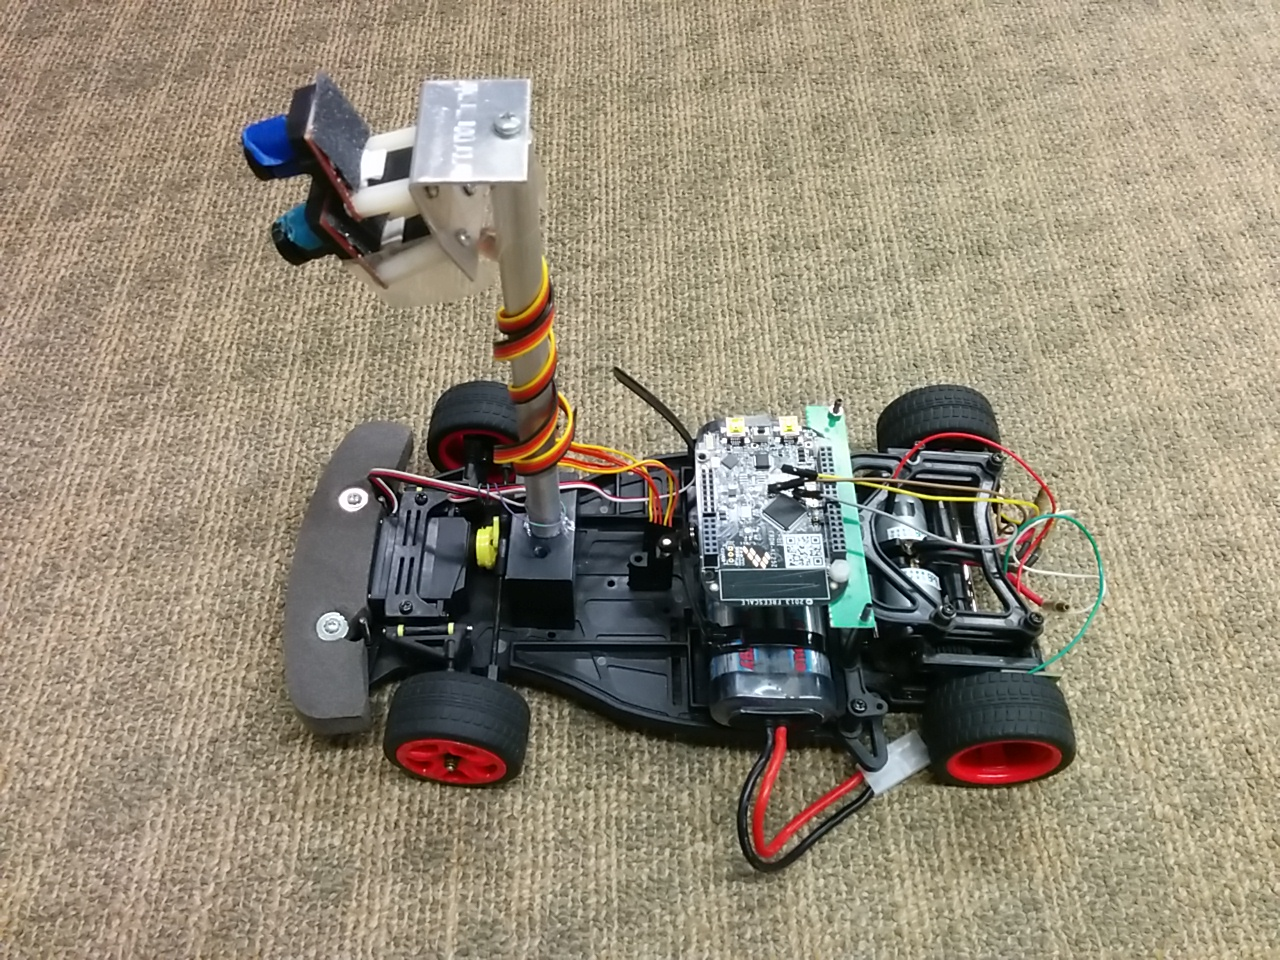
\includegraphics[width=0.32\textwidth]{images-dis2-carcritiques/barecar-side1}
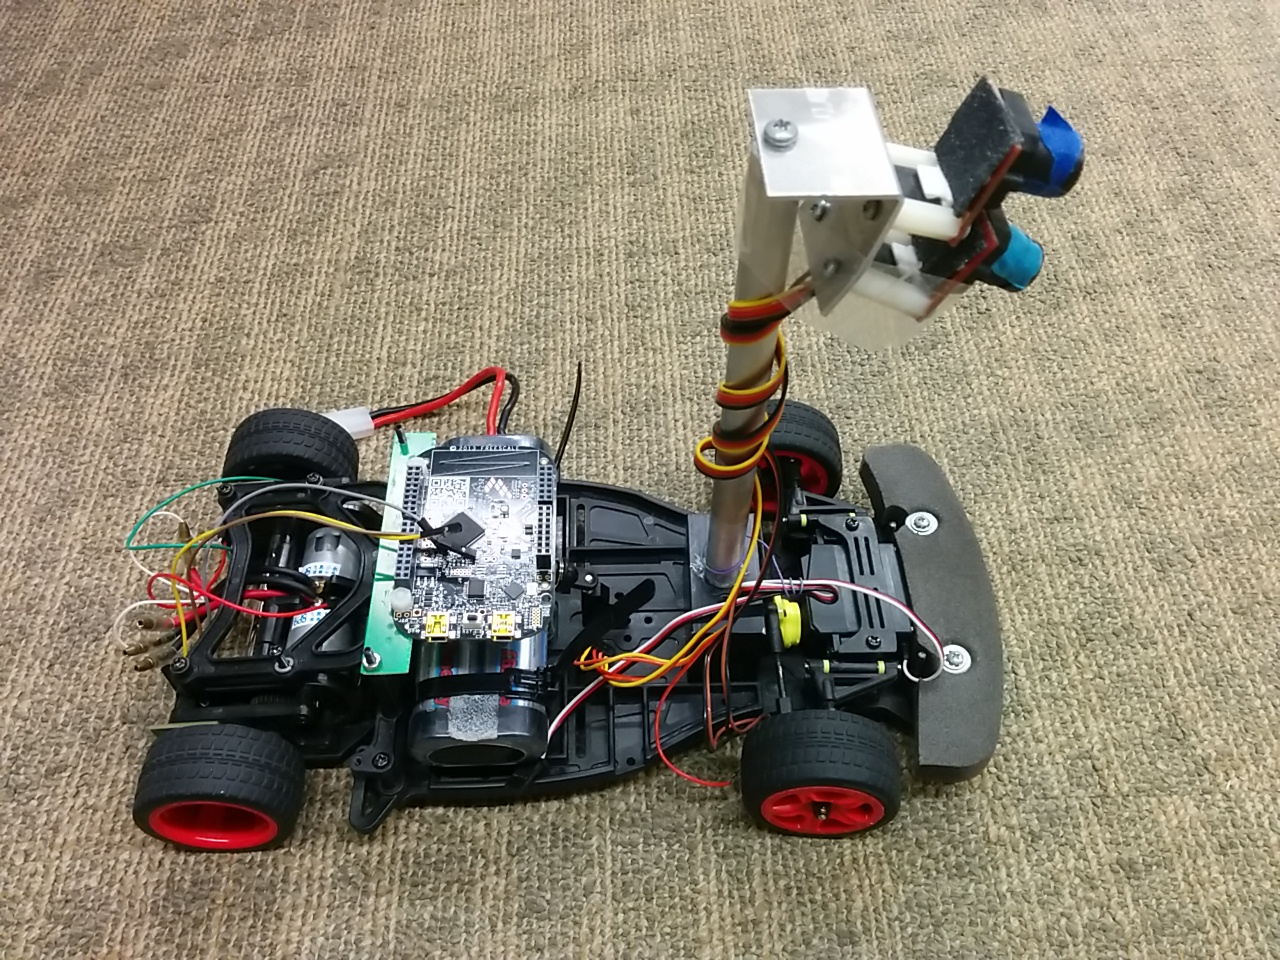
\includegraphics[width=0.32\textwidth]{images-dis2-carcritiques/barecar-side2}
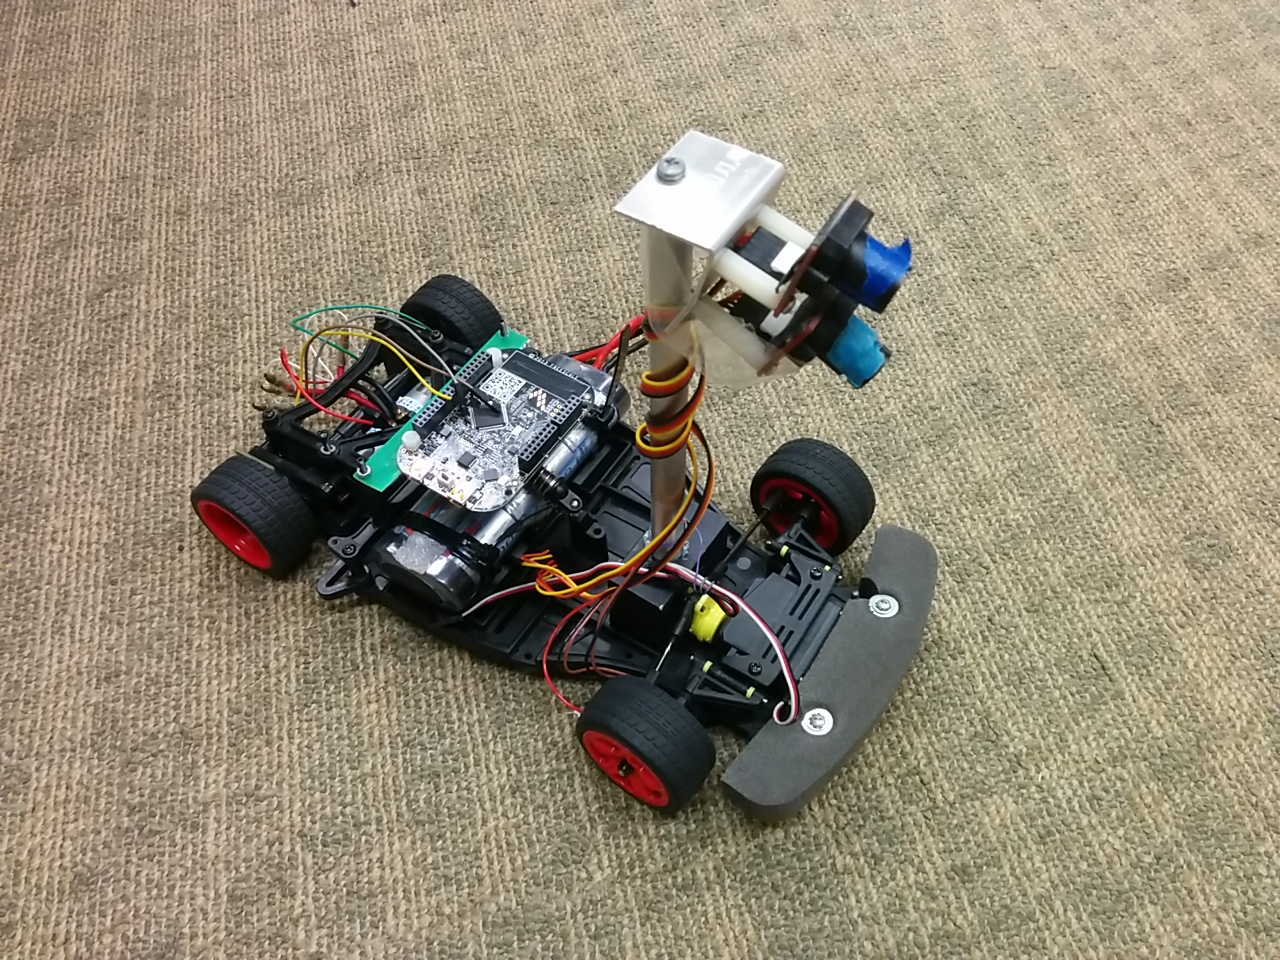
\includegraphics[width=0.32\textwidth]{images-dis2-carcritiques/barecar-angle} \\
\textit{I guess the team just liked their circuit boards that much and decided to keep them...} \\
There really wasn't much to say here, since there wasn't much to look at. \\}

\begin{tabularx}{\textwidth}{X X}
\textbf{Did well} & \textbf{Could improve} \\
\begin{itemize}
  \item Very rigid camera mount, but might also have been excessive (solid aluminum brick)
\end{itemize}
&
\begin{itemize}
  \item Lots of loose connectors, none of them have been ziptied down or together
  \item The angled bracket camera mount may have been experiencing stability issues - cameras are taped down
  \item FRDM-KL25Z board insecurely mounted - cantilevered - may experience stability issues and can cause intermittent connector interruptions
  \item ... so don't even THINK about using the accelerometer ...
\end{itemize}
\end{tabularx}

\subsection{Team So Good's Car}
{\centering
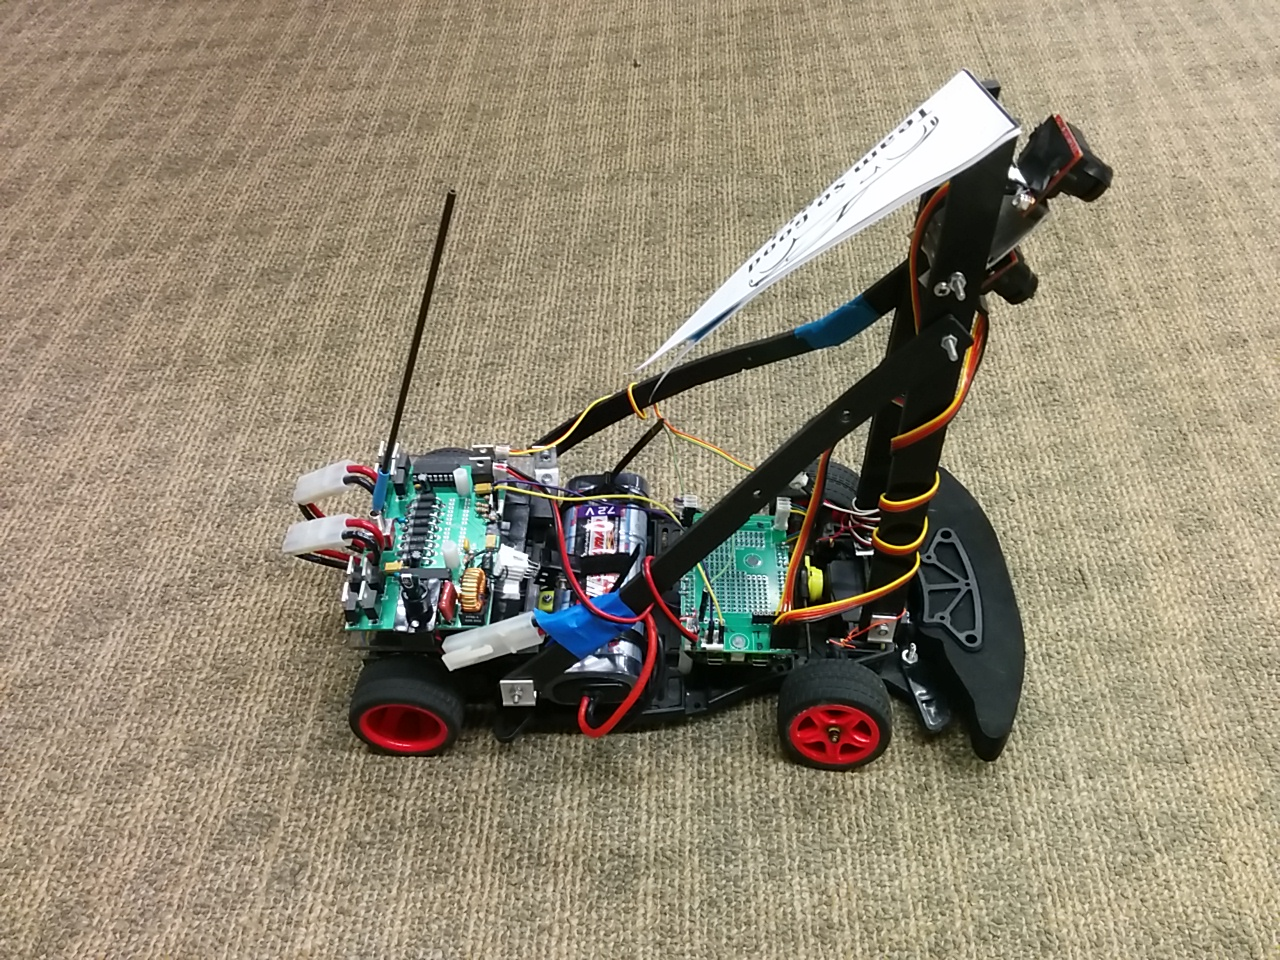
\includegraphics[width=0.32\textwidth]{images-dis2-carcritiques/sogood-side1}
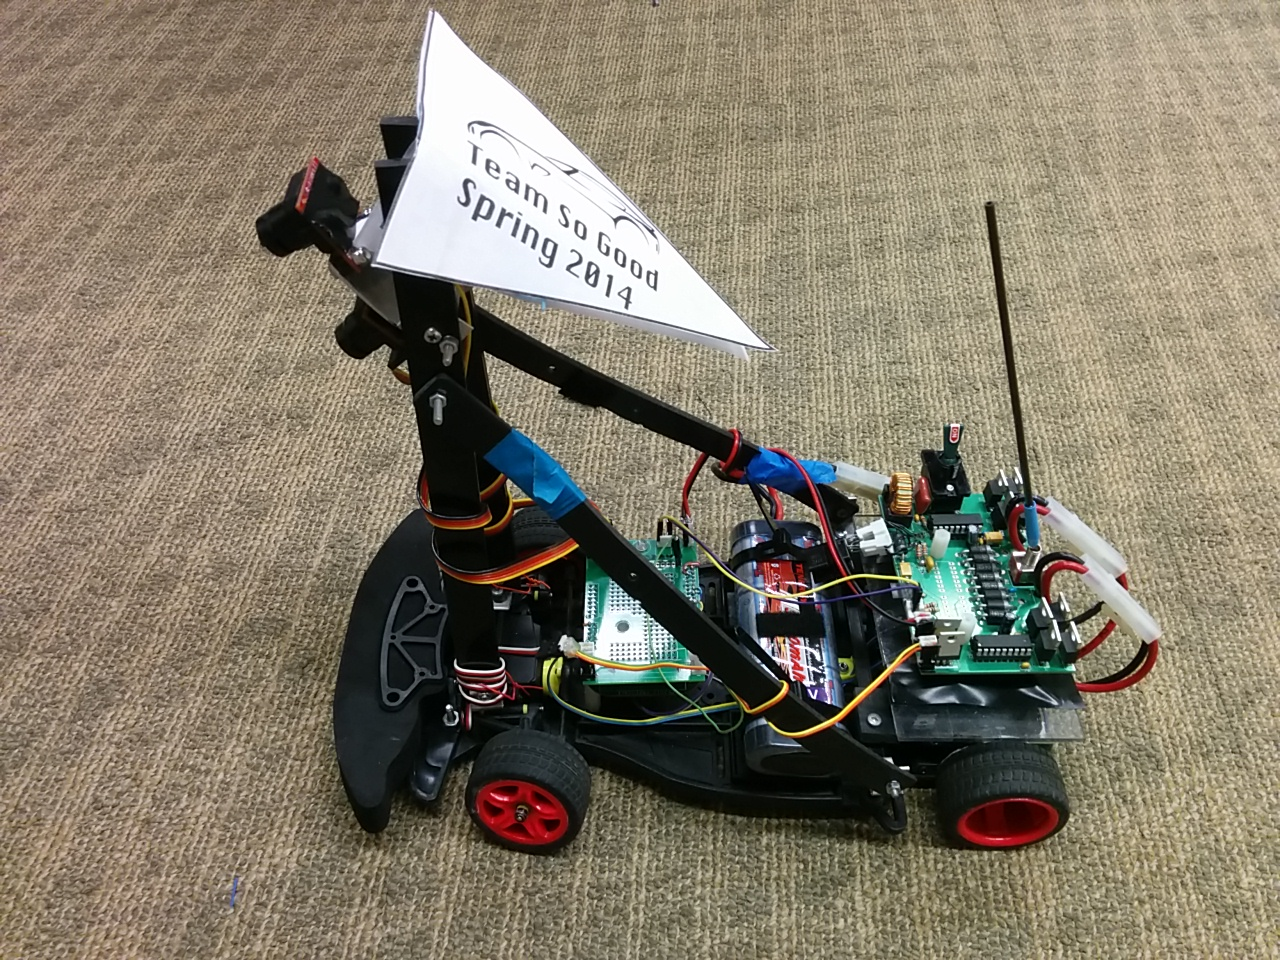
\includegraphics[width=0.32\textwidth]{images-dis2-carcritiques/sogood-side2}
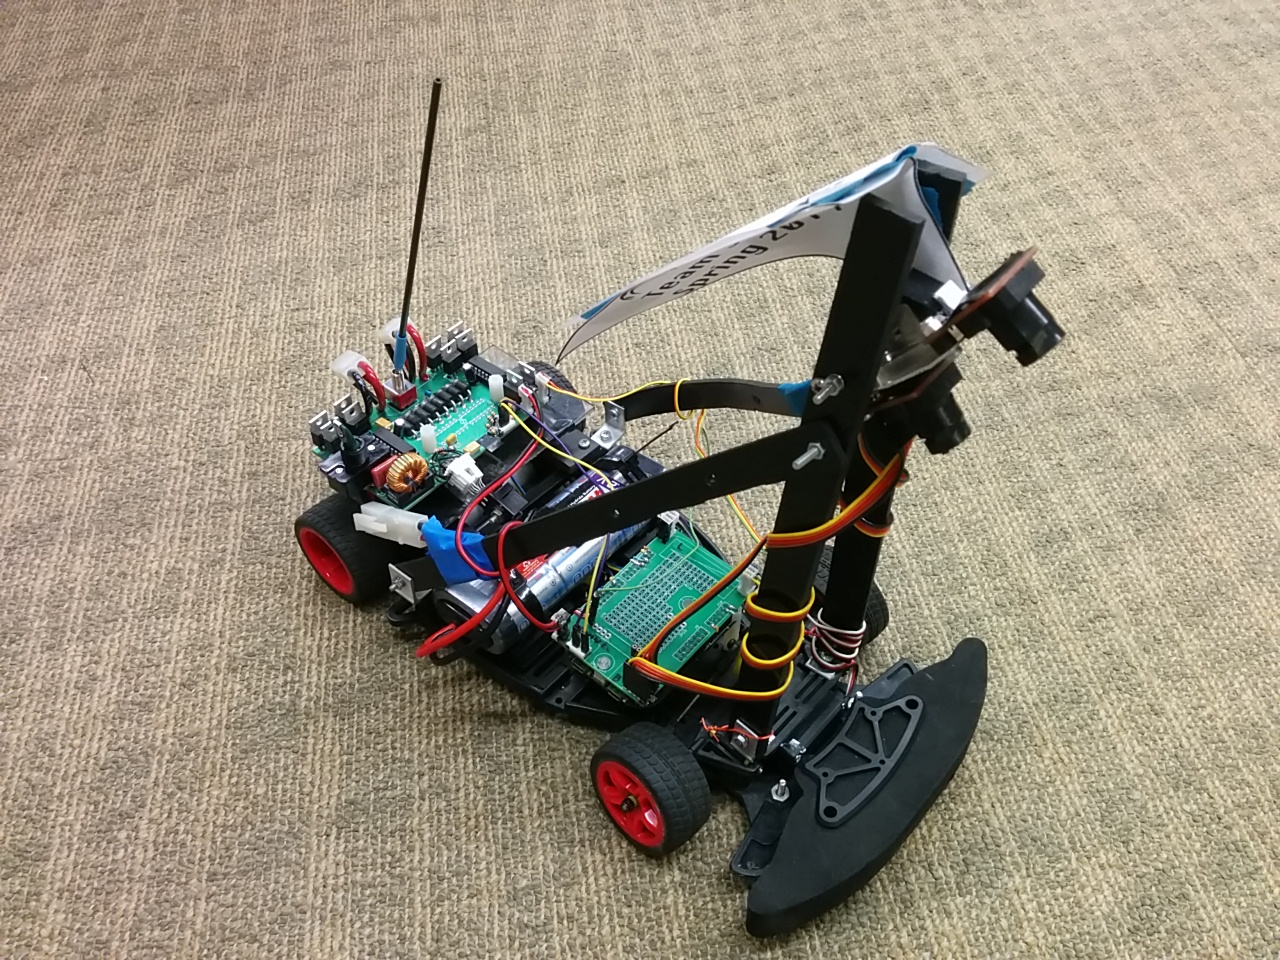
\includegraphics[width=0.32\textwidth]{images-dis2-carcritiques/sogood-angle} \\
\textit{Actually going to end up (intact) in the 192 display case someday - so they obviously did something right} \\}

\begin{tabularx}{\textwidth}{X X}
\textbf{Did well} & \textbf{Could improve} \\
\begin{itemize}
  \item Clean and compact board design
  \item FRDM shield PCB: only a few connectors, all with polarized MTA (the IDC-type connectors) connectors
  \item Large safety stop switch to smack
  \item Battery extra-secured with velcro
  \item Good camera mount with a triangular frame, uses lightweight plastic for frame while using only smaller metal pieces for extra stability
  \item Design for Test: shield PCB may expose all the pins (it's unclear what exactly the through-hole array on the board does, but it may break out all the MCU pins)
  \item Camber on the front wheels (if you look at it from the front, they are angled outwards towards the bottom) - this helps cornering performance - if the car starts to tilt, the wheels get more contact area and traction
  \item Hot-glue to insulate solder joints (or for extra connector security)
  \item Connectors have been colored to indicate polarity (as if the polarizing tab wasn't enough)
  \item Board labeled with which camera goes where
\end{itemize}
&
\begin{itemize}
  \item Lots of fasteners can be a failure point (but seems secured with lock washers)
  \item Some wire-to-board solder joints - may have been blue-wire fixes
  \item Floating DC-DC converter chip (``socketed'' with two MTA connectors, connected to the PCB with wire-to-board solder joints)
  \item MOSFETs (motor driver transistors, a lot of current goes through these things in operation!) vulnerable to physical damage by placement - may even short to each other if kicked
  \item No heatsinking provisions for MOSFETs
  \item Why was the board mounted so far backwards? Sensitive electronics more vulnerable to kicking
\end{itemize}
\end{tabularx}

\section{Thursday, 28 January}
\subsection{Wood Brick Camera Car}
{\centering
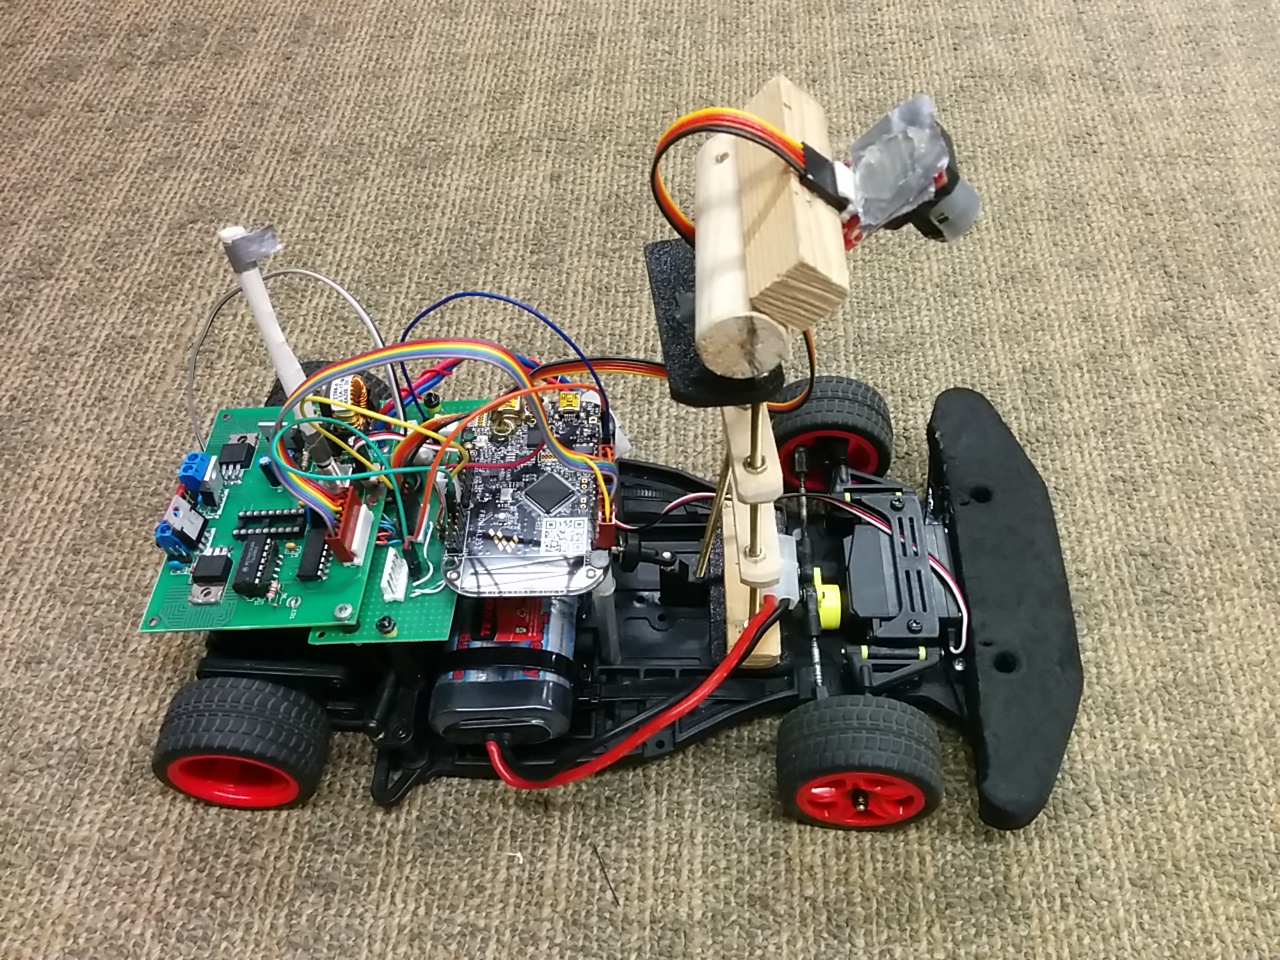
\includegraphics[width=0.32\textwidth]{images-dis2-carcritiques/brickcar-side1}
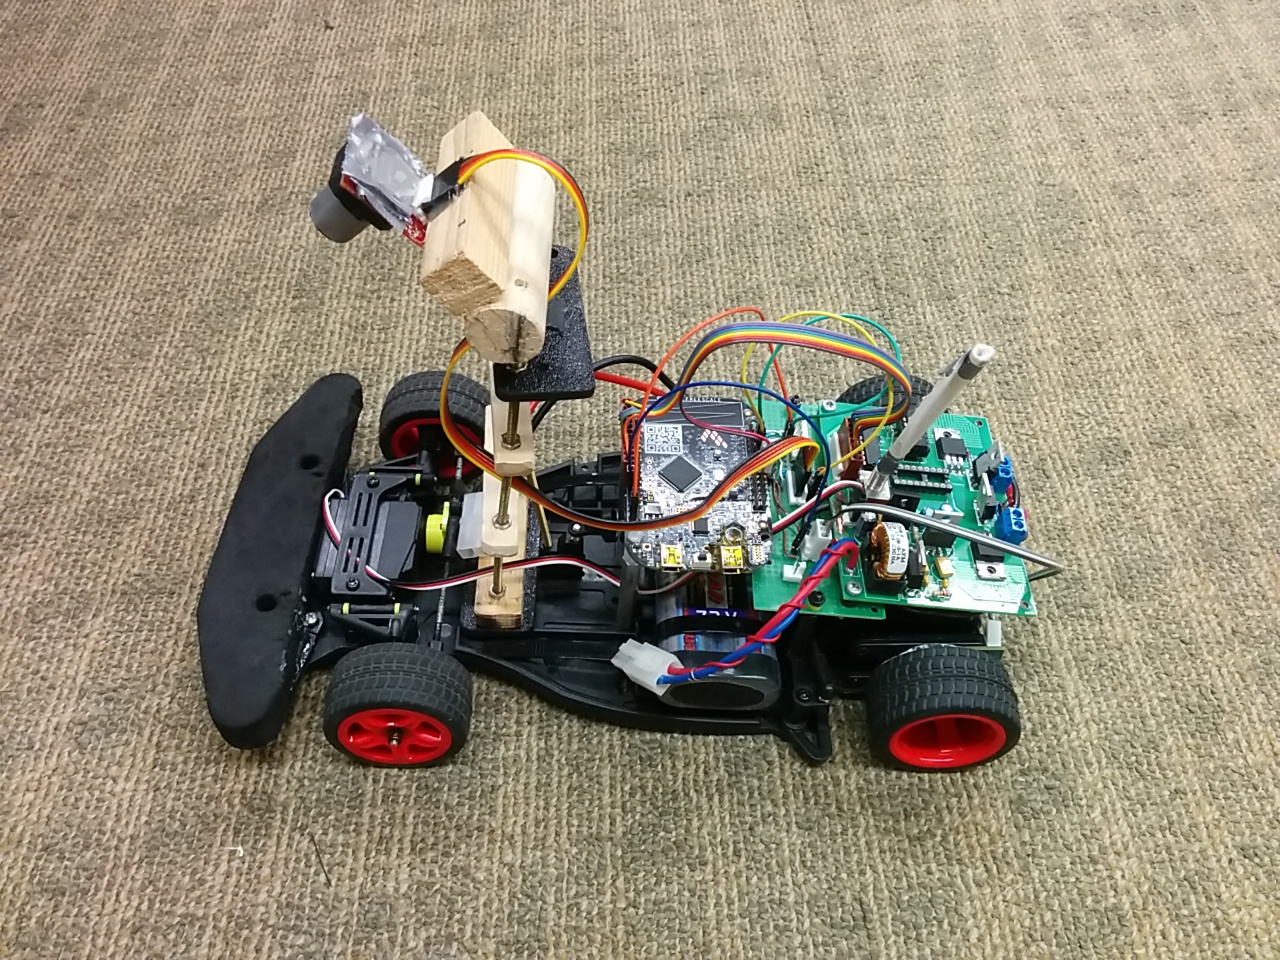
\includegraphics[width=0.32\textwidth]{images-dis2-carcritiques/brickcar-side2}
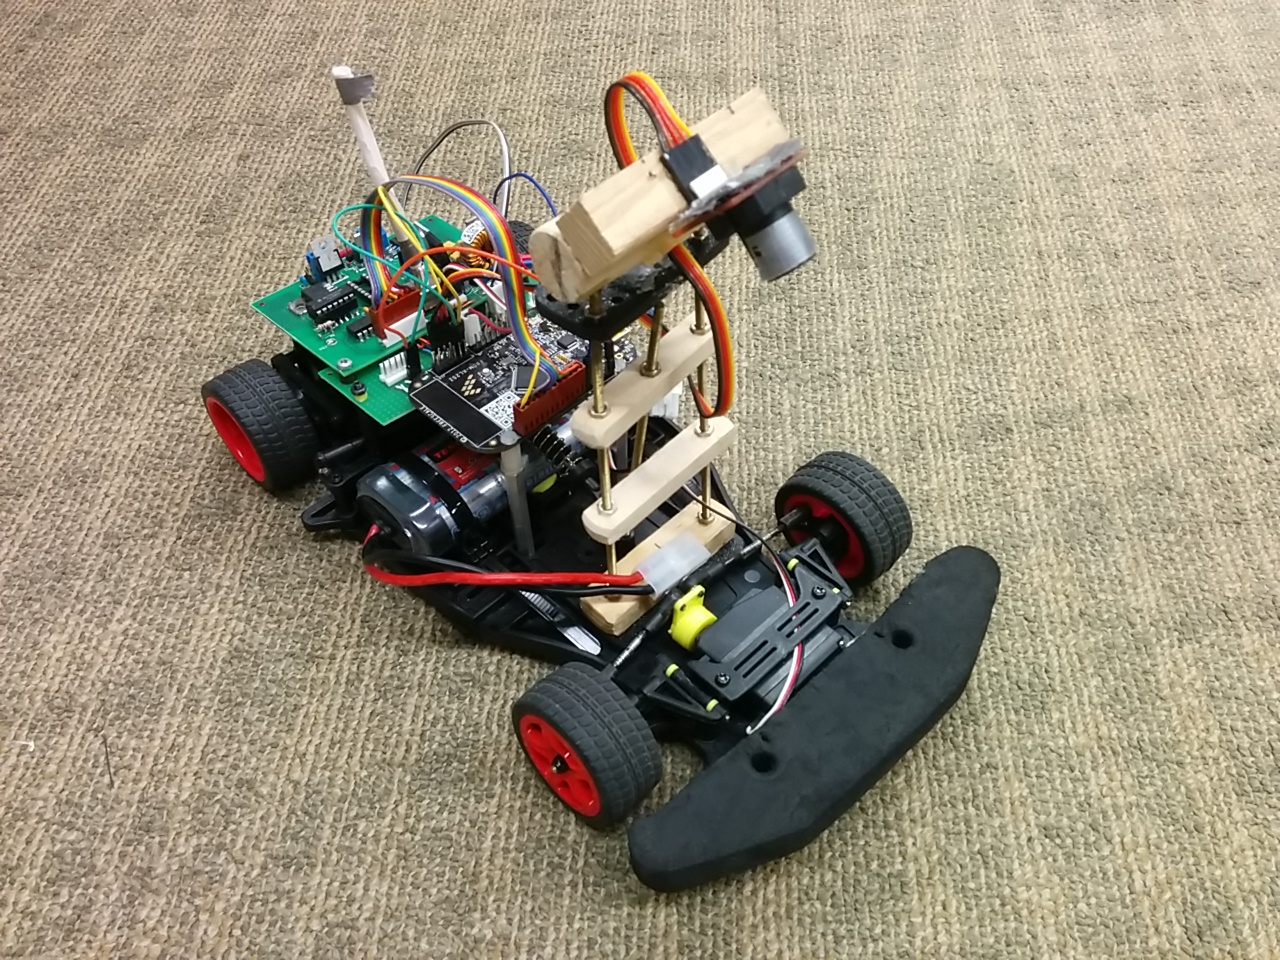
\includegraphics[width=0.32\textwidth]{images-dis2-carcritiques/brickcar-angle} \\}

\begin{tabularx}{\textwidth}{X X}
\textbf{Did well} & \textbf{Could improve} \\
\begin{itemize}
  \item Heatshrink on wire solder joints
  \item PCB layout is pretty neat, you can see what's going on

\end{itemize}
&
\begin{itemize}
  \item Screwed up on a lot of places - there is epoxy on the FRDM-KL25Z board
  \item Mechanical design was ``abysmal'' (literally what was said during discussion) - a lot of weight placed high up means a high center of gravity
  \item Nothing was put on the front of the chassis - likely done for simplicity - but should think more about overall design
  \item Nothing is oiled, high friction on moving parts
\end{itemize}
\end{tabularx}

\subsection{Protoboard Car}
{\centering
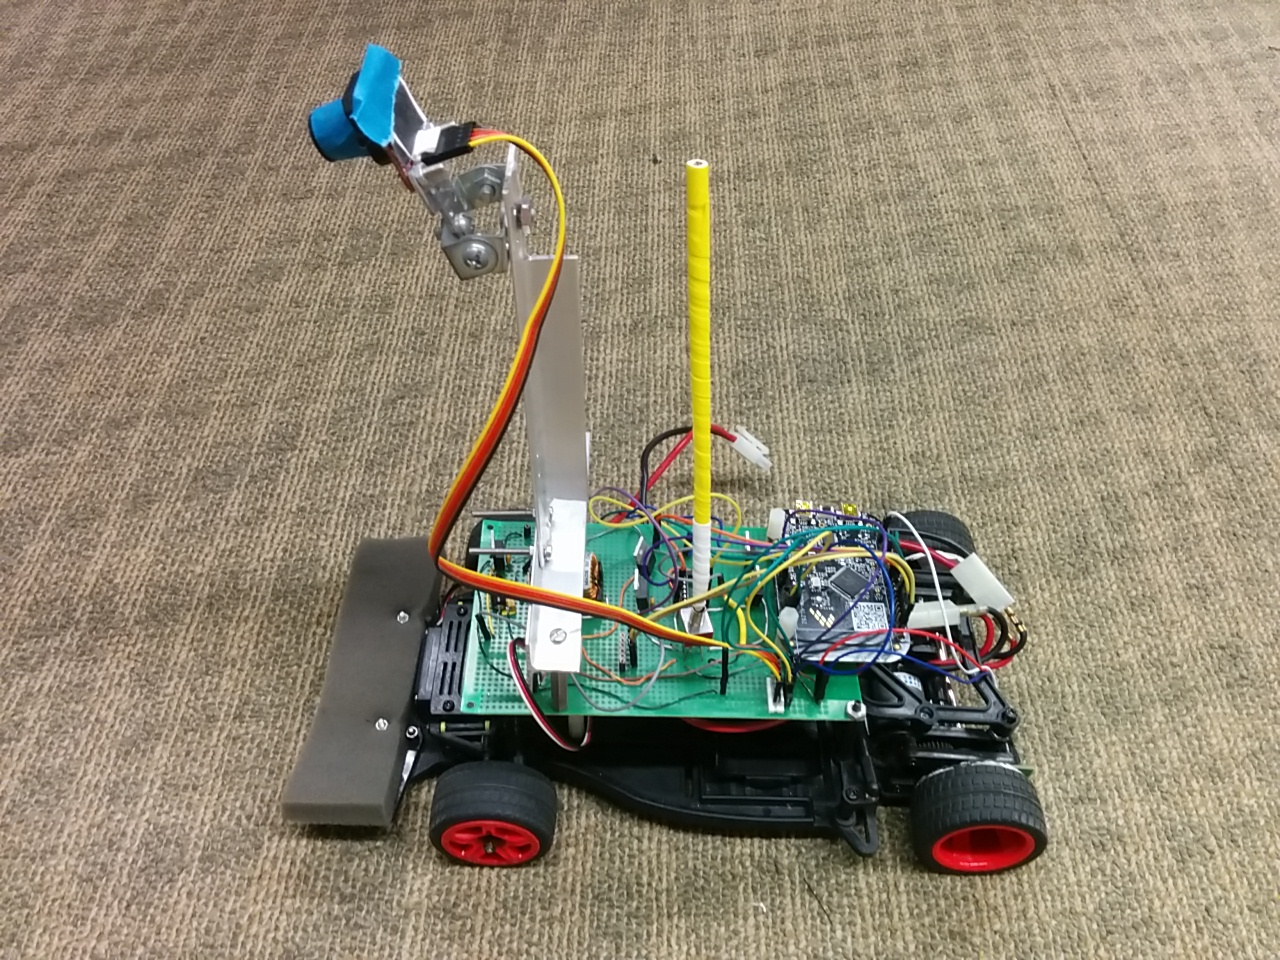
\includegraphics[width=0.32\textwidth]{images-dis2-carcritiques/protoboard-side1}
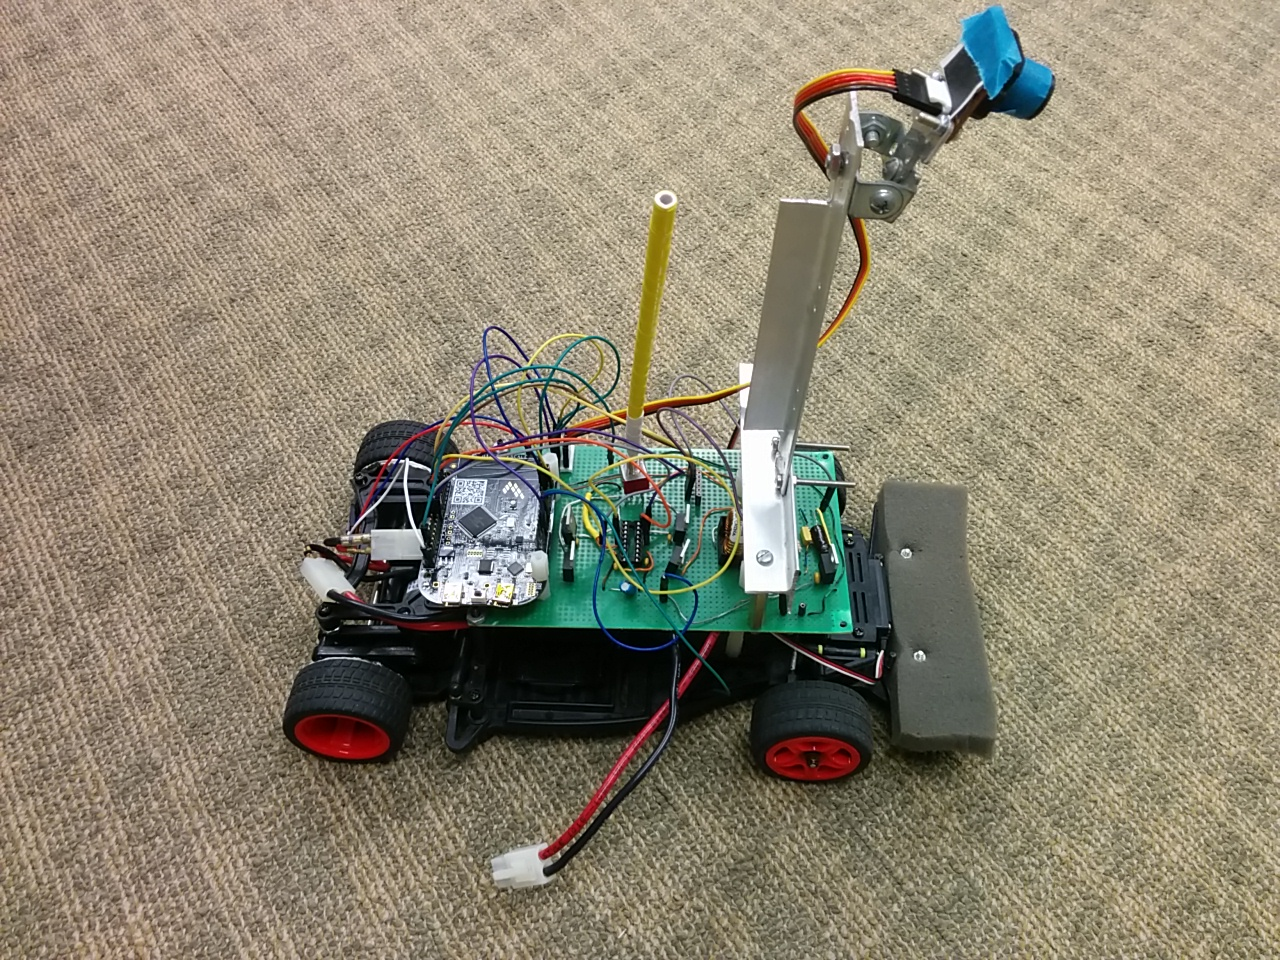
\includegraphics[width=0.32\textwidth]{images-dis2-carcritiques/protoboard-side2}
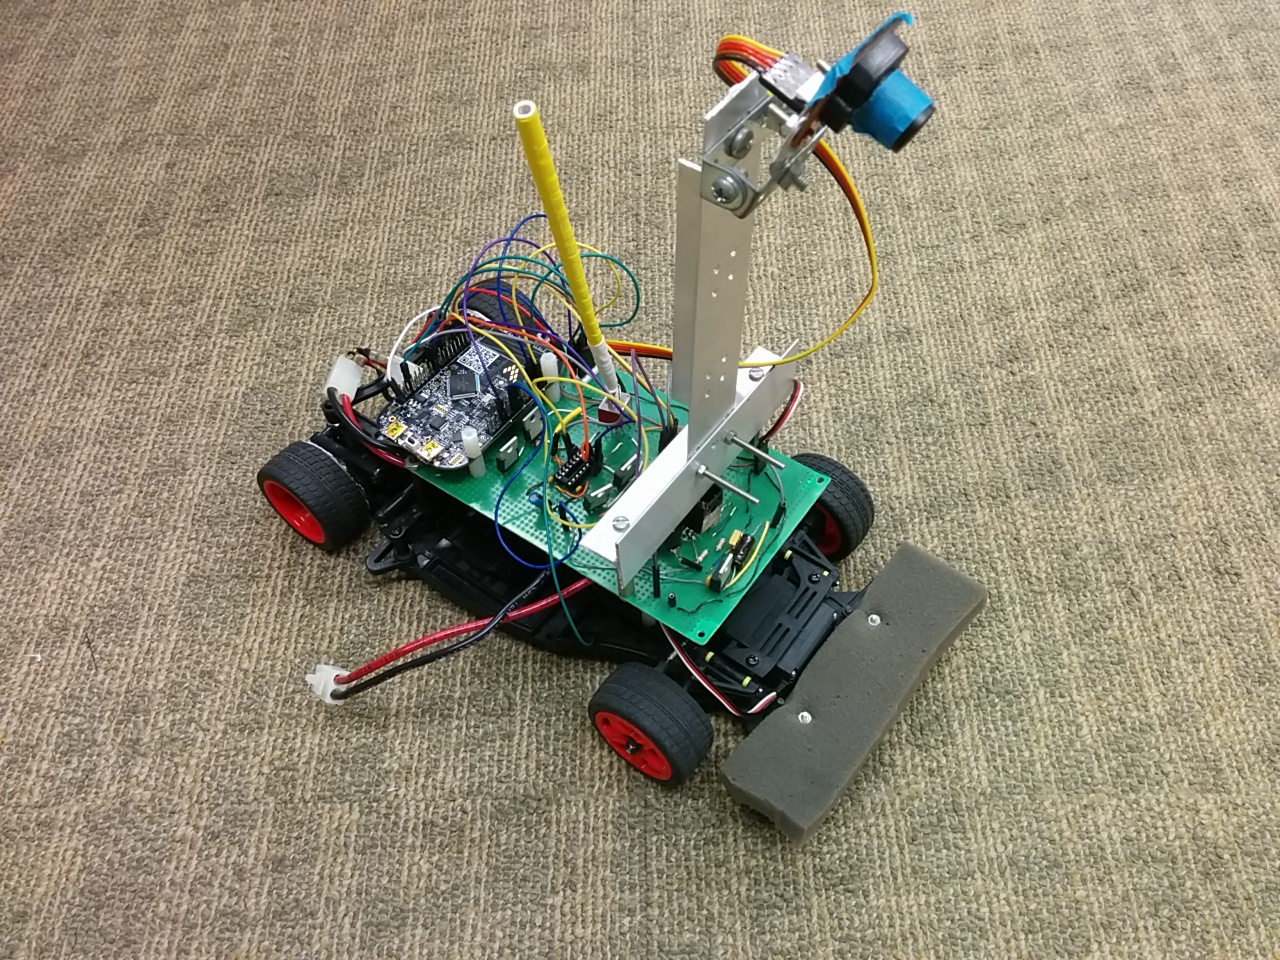
\includegraphics[width=0.32\textwidth]{images-dis2-carcritiques/protoboard-angle} \\}

\begin{tabularx}{\textwidth}{X X}
\textbf{Did well} & \textbf{Could improve} \\
\begin{itemize}
  \item Adjustable camera-to-mast mounting mechanism (might just re-use those parts...)
  \item Speed sensing mechanism is nice: IR reflector onto codewheel mounted on wheel
  \item \textit{Instructor's note: you'll see a similar sensor mechanism mounted to many cars - the board was designed by ESG and is available to all teams}
\end{itemize}
&
\begin{itemize}
  \item Metal camera mast is heavy
  \item Camera mast metal geometry (T-bar) provides stiffness for most of the mast ... EXCEPT the base where it matters (in fact, the mast is bolted to the PCB, so the PCB is now a structural component)
  \item Handmade protoboard - worries about shorting
  \item Super soft front foam bumper, might not actually do much in a crash
  \item Power connectors are coming out of their sockets
  \item Janky flag mount
  \item Many screws loose, things aren't bolted on quite right
  \item Just kind of ugly overall...
\end{itemize}
\end{tabularx}

\subsection{Another Car}
{\centering
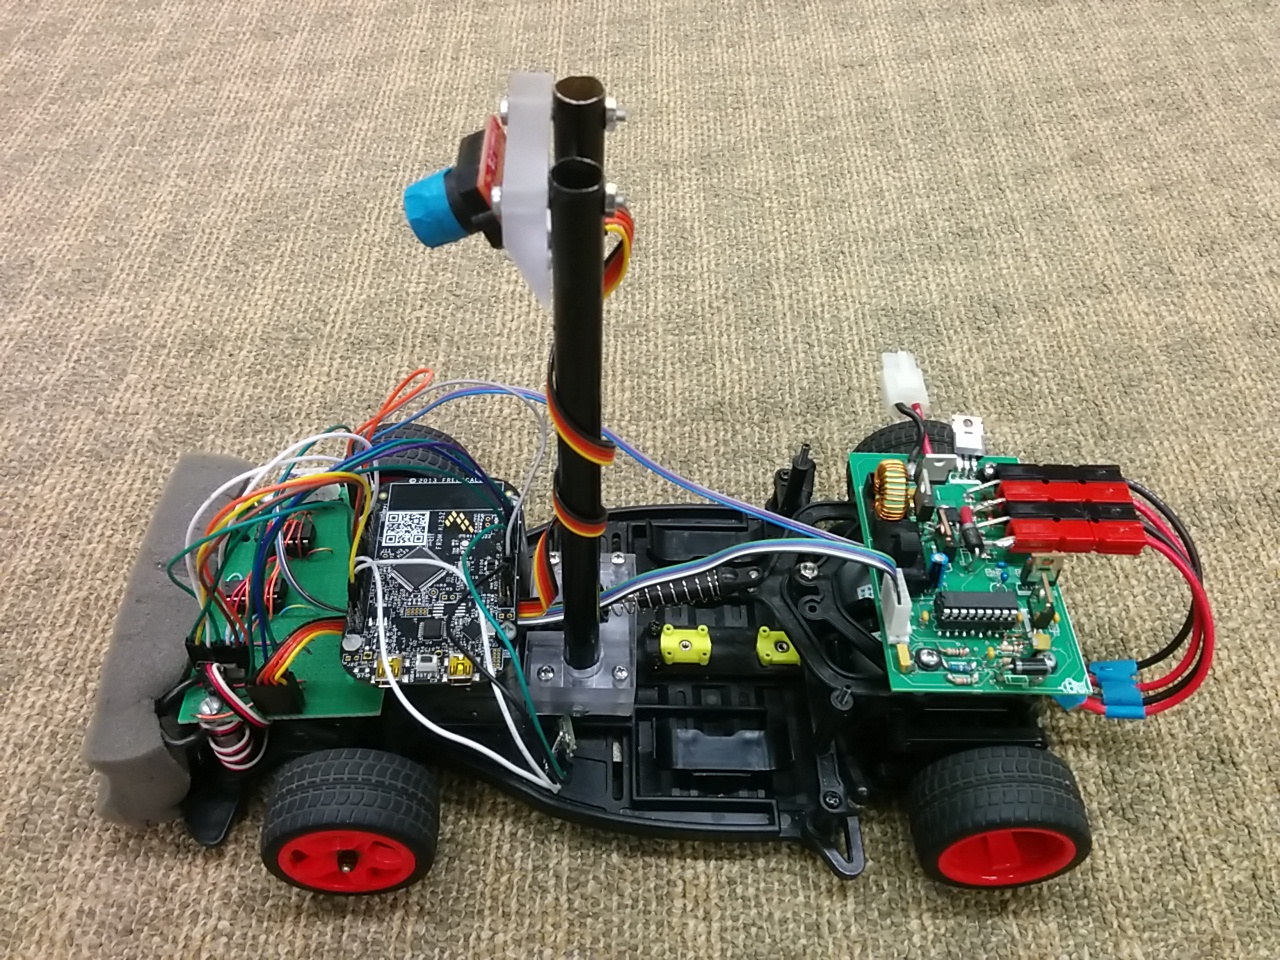
\includegraphics[width=0.32\textwidth]{images-dis2-carcritiques/thecar-side1}
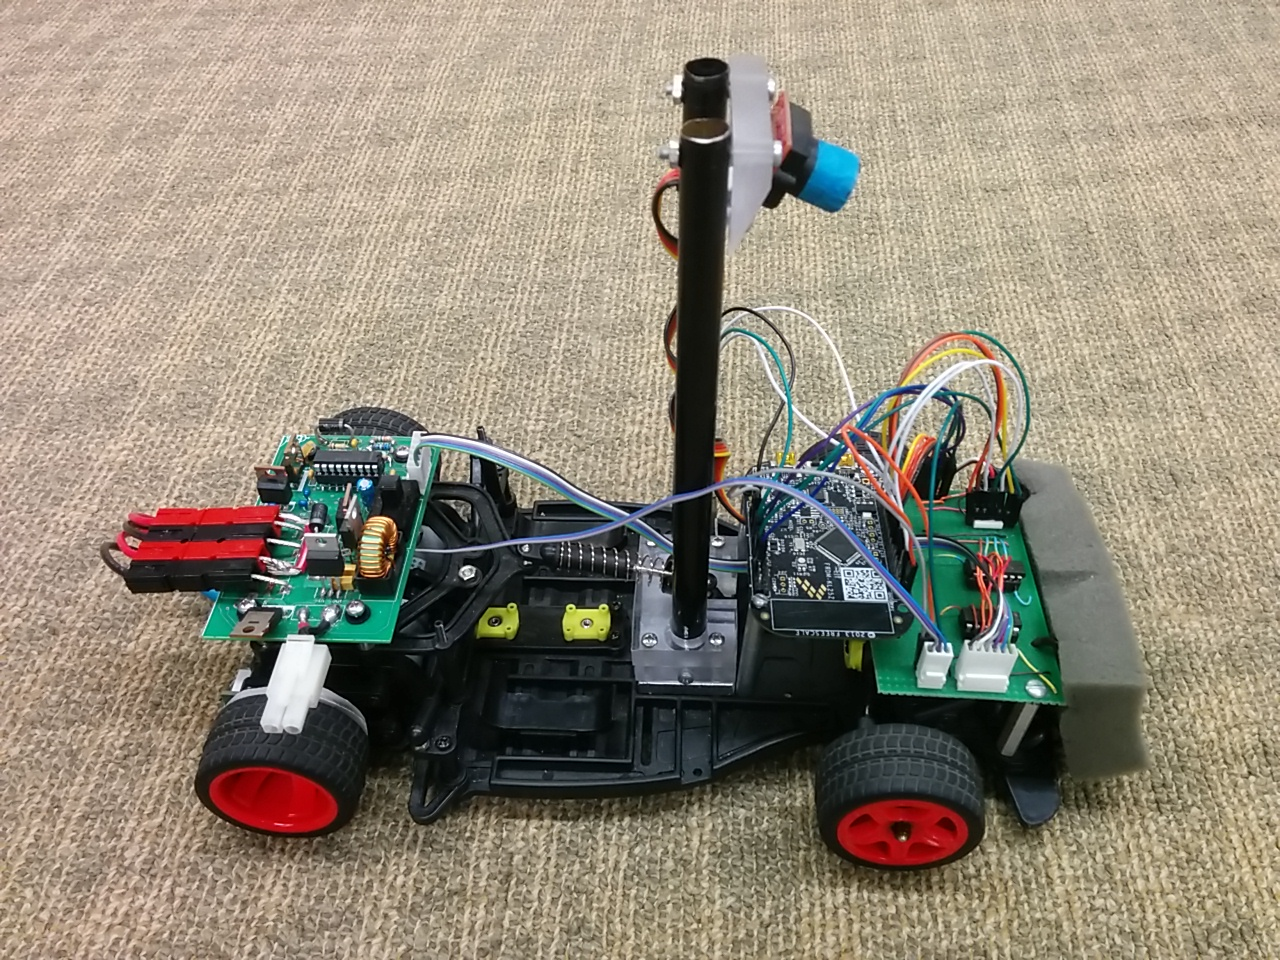
\includegraphics[width=0.32\textwidth]{images-dis2-carcritiques/thecar-side2}
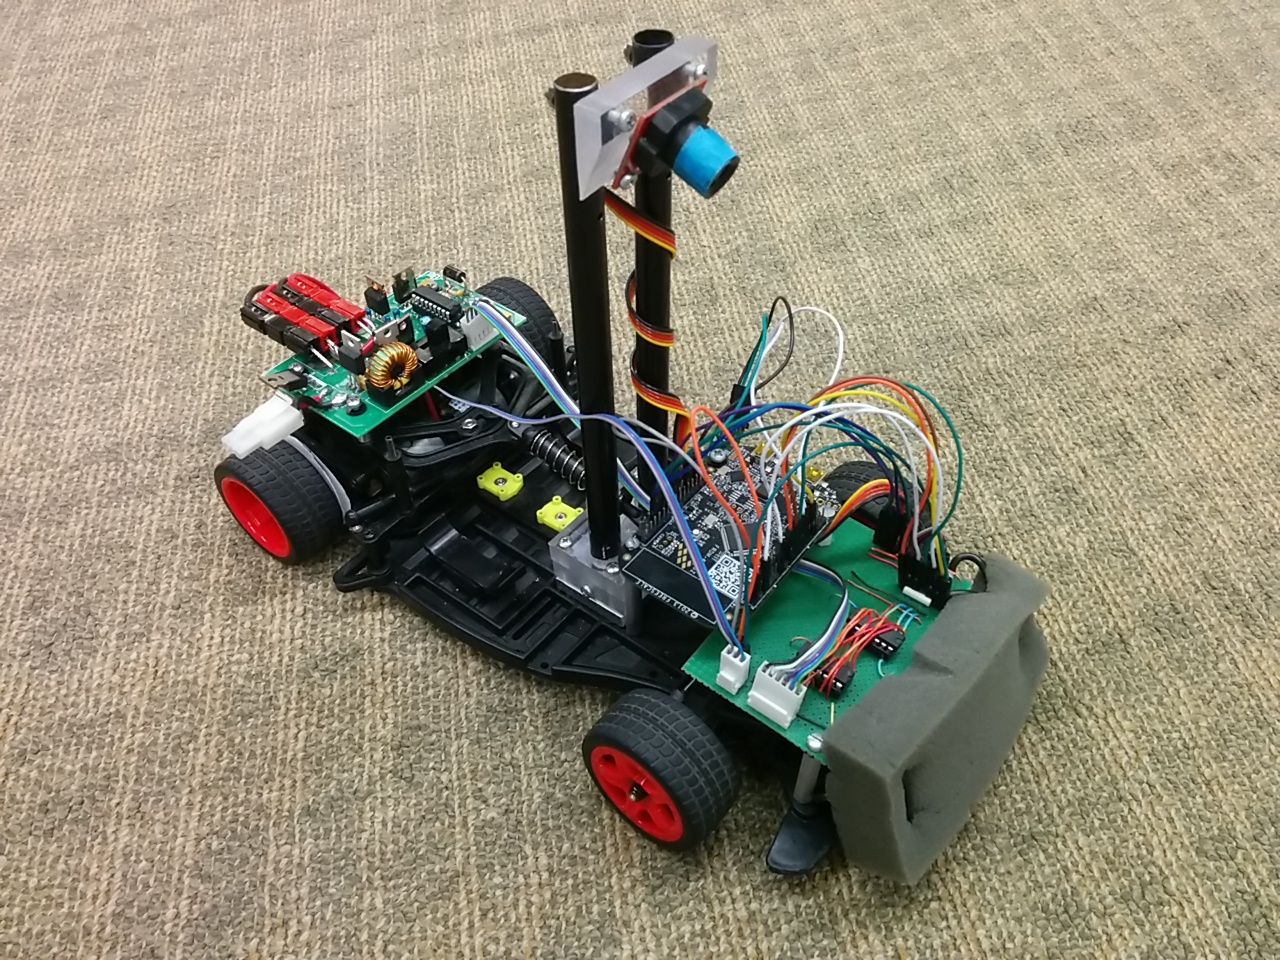
\includegraphics[width=0.32\textwidth]{images-dis2-carcritiques/thecar-angle} \\
\textit{I really can't think of a creative and unique name for this right now...} \\}

\begin{tabularx}{\textwidth}{X X}
\textbf{Did well} & \textbf{Could improve} \\
\begin{itemize}
  \item Fairly stable camera mount
  \item At least they HAD a Bluetooth module
  \item Anderson connectors
  \item \textit{Instructor's note: Anderson PowerPole connectors will be made standard for the class this year, replacing the Tamiya connectors which some teams have had issues with}
  \item Encoder is decently mounted
  \item Big power switch on the board is in a nice location
  \item Really nice camera mount, looks like it received a lot of attention (the mast is made of hollow metal tubes)
\end{itemize}
&
\begin{itemize}
  \item Non-adjustable camera mount - either got it really right the first time, or in serious trouble
  \item Terrible soldering jobs, no surface mount
  \item \textit{Instructor's note: use of surface-mount components is more common in industry due to compactness and better compatibility with automated processes. You're free to use SMT for ee192 if you're comfortable with soldering these components, but we'll give you enough board area to do an all-through-hole design.}
  \item All the SMT tantalum capacitors are deadbugged (capacitors are on their sides, soldered down to pins instead of a surface-mount pad - likely a way to fit SMT components onto a through-hole pad)
  \item Questionable mechanical stability of the FRDM board, just by the number of wires sticking out of it
  \item Floating Bluetooth module
  \item Really, their protoboard is nicer than their PCB
\end{itemize}
\end{tabularx}

\subsection{Nyancat Nyancar}
{\centering
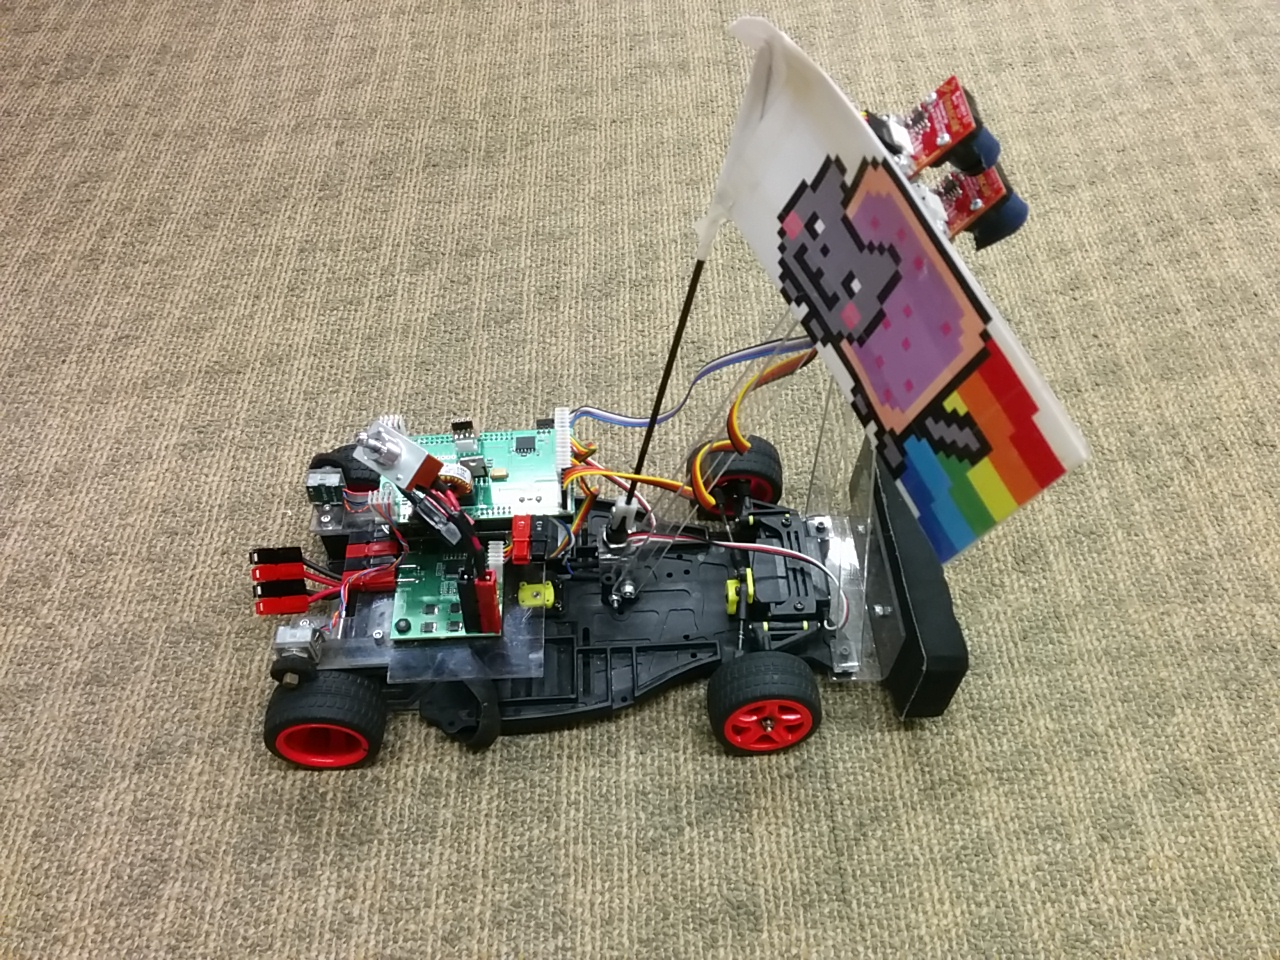
\includegraphics[width=0.32\textwidth]{images-dis2-carcritiques/nandcar-side1}
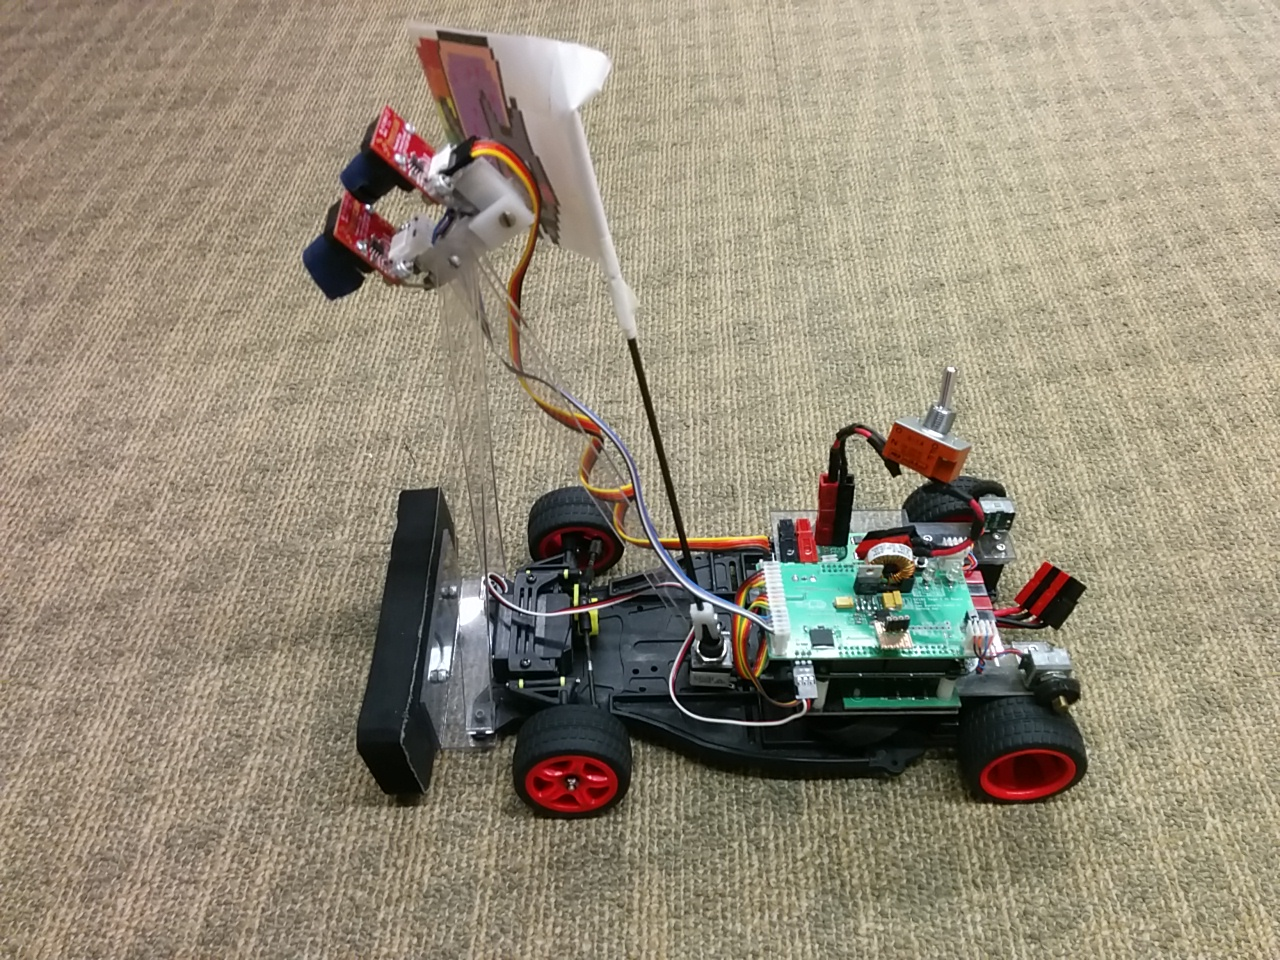
\includegraphics[width=0.32\textwidth]{images-dis2-carcritiques/nandcar-side2}
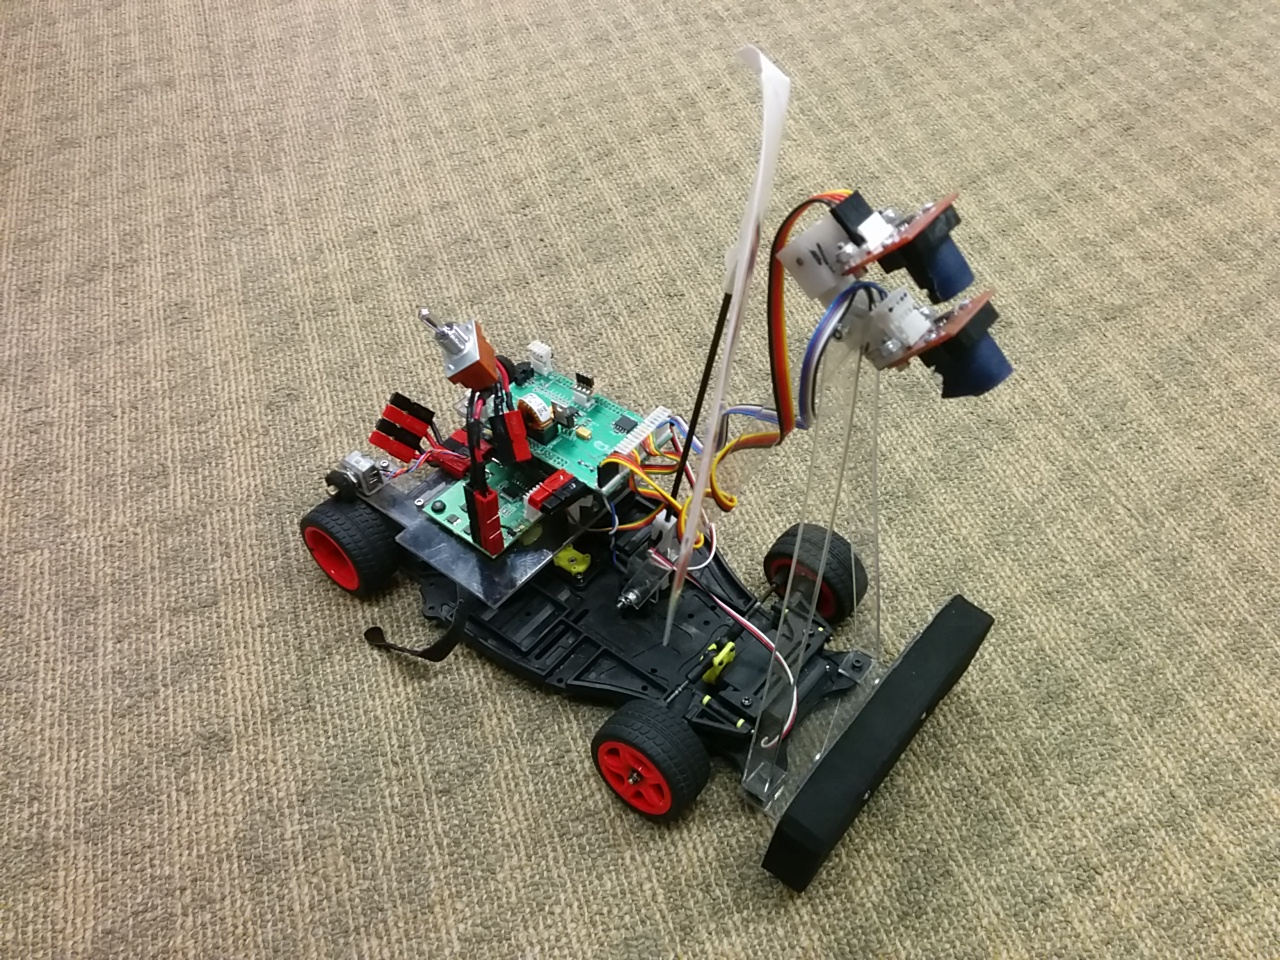
\includegraphics[width=0.32\textwidth]{images-dis2-carcritiques/nandcar-angle} \\}

\begin{tabularx}{\textwidth}{X X}
\textbf{Did well} & \textbf{Could improve} \\
\begin{itemize}
  \item Good PCB design
  \item Battery secured with Velcro straps, making it easy to install and take out
  \item Camera mast is decent, though there are still some stability issues
  \item Lightweight but robust plastic for triangular camera mast
  \item Some degree of adjustability for cameras
  \item Clean wiring between boards - lack of visible wires
  \item Neat overall
  \item Liked flag connected to kill switch
\end{itemize}
&
\begin{itemize}
  \item Not-so-good SMT soldering skills
\end{itemize}
\end{tabularx}

\end{document}

